\chapter{B-2 Construction of a stadium}

A town council wishes to construct a small stadium in order to improve the
services provided to the people living in the district. After the invitation to
tender, a local construction company is awarded the contract and wishes
to complete the task within the shortest possible time. All major tasks are
listed in the following table. The durations are expressed in weeks. Some tasks
can only start after the completion of certain other tasks. The last two
columns of the table refer to question 2 which we shall see later.

\textbf{Question 1:} What is the earliest possible date of completing the
construction?

\textbf{Question 2:} The town council would like the project to terminate earlier
than the time announced by the builder (answer to question 1). To obtain this,
the council is prepared to pay a bonus of $\euro{}30\mathrm{K}$ for every week the work
finishes early. The builder needs to employ additional workers and rent more
equipment to cut down on the total time. In the preceding table he has 
summarized the maximum number of weeks he can save per task (column "Max. reduct.")
and the associated additional cost per week. When will the project be completed
if the builder wishes to maximize his profit?

\newpage

\section{Question 1}

\subsection{Parameters}

\begin{syms}
\item[$T$] enumerates $n=18+1$ project tasks, ie. $T=\left\lbrace 1,\ldots, n+1\right\rbrace$

\item[$A$] the matrix of arcs with $A\in\left\lbrace 0,1\right\rbrace^{n+1\times n+1}$;
    with elements $a_{ij}=\begin{cases}1 & \texttt{task } j \text{ preceeds }\texttt{task }i\\
    0 & \text{otherwise}\end{cases}$

\item[$d_t$] the duration in weeks to complete task $t\in T$ with no additional labour hours allocated

\end{syms}

\textbf{Note:} A ficticious task \texttt{Done} with $t=19$ and $d_{19}=0$ is also added which has all other
terminal tasks as predecessors.

\subsubsection{Data given for parameters}

\begin{table}[h]
    \center
    \caption{Data for stadium construction}\label{table:1-1}
    {\small
    \begin{tabu}{clcccc}
        \hline
        \rowfont[c]{\bfseries} Task & Description & Duration $d_t$ & Predecessors $P_t$ & Max. reduct. $r_t$ & Add. cost $c_t$ \\
        \hline
        {\bfseries 1} & Installing the construction site & 2 & - & 0 & - \\
        {\bfseries 2} & Terracing  & 16 & 1 & 3 & 30 \\
        {\bfseries 3} & Constructing the foundations & 9 & 2 & 1 & 26 \\
        {\bfseries 4} & Access roads and other networks  & 8 & 2 & 2 & 12 \\
        {\bfseries 5} & Erecting the basement  & 10 & 3 & 2 & 17 \\        
        {\bfseries 6} & Main floor  & 6 & 4, 5 & 1 & 15 \\
        {\bfseries 7} & Dividing up the changing rooms  & 2 & 4 & 1 & 8 \\
        {\bfseries 8} & Electrifying the terraces  & 2 & 6 & 0 & - \\
        {\bfseries 9} & Constructing the roof  & 9 & 4, 6 & 2 & 42 \\
        {\bfseries 10} & Lighting of the stadium  & 5 & 4 & 1 & 21 \\
        {\bfseries 11} & Installing the terraces  & 3 & 6 & 1 & 18 \\
        {\bfseries 12} & Sealing the roof  & 2 & 9 & 0 & - \\
        {\bfseries 13} & Finishing the changing rooms  & 1 & 7 & 0 & - \\
        {\bfseries 14} & Constructing the ticket office  & 7 & 2 & 2 & 22 \\
        {\bfseries 15} & Secondary access roads  & 4 & 4, 14 & 2 & 12 \\
        {\bfseries 16} & Means of signalling  & 3 & 8, 11, 14 & 1 & 6 \\
        {\bfseries 17} & Lawn and sport acessories  & 9 & 12 & 3 & 16 \\
        {\bfseries 18} & Handing over the building  & 1 & 17 & 0 & - \\
        \hline
                       &\\
    \end{tabu}
}
    \emph{Note:} Columns $r_t$ and $c_t$ is not used for question 1.
\end{table}

\newpage

\subsubsection{Task precedence}

Some task $t\in T$ may have a predecessor $p\in T$. In other words task $t$ can not
commence until task $p$ is finished. In this example, ``Erecting the basement'' can
not be begun until after ``Constructing the foundation'' completes.

For some task $t\in T$, it has predecessors as the set 
$P_t = \left\lbrace p_{t0}, \ldots, p_{tk} : p_{tk} \in T \text{ and }
    p_{tk} \text{ preceeds } p_{t0} \right\rbrace$. Note that we could have
    $P_t = \emptyset$. One may visualize this graph as in \cref{figure:1-1}.


\begin{figure}[h]
    \center
    \caption{Graph of precedence dependencies of tasks}\label{figure:1-1}
    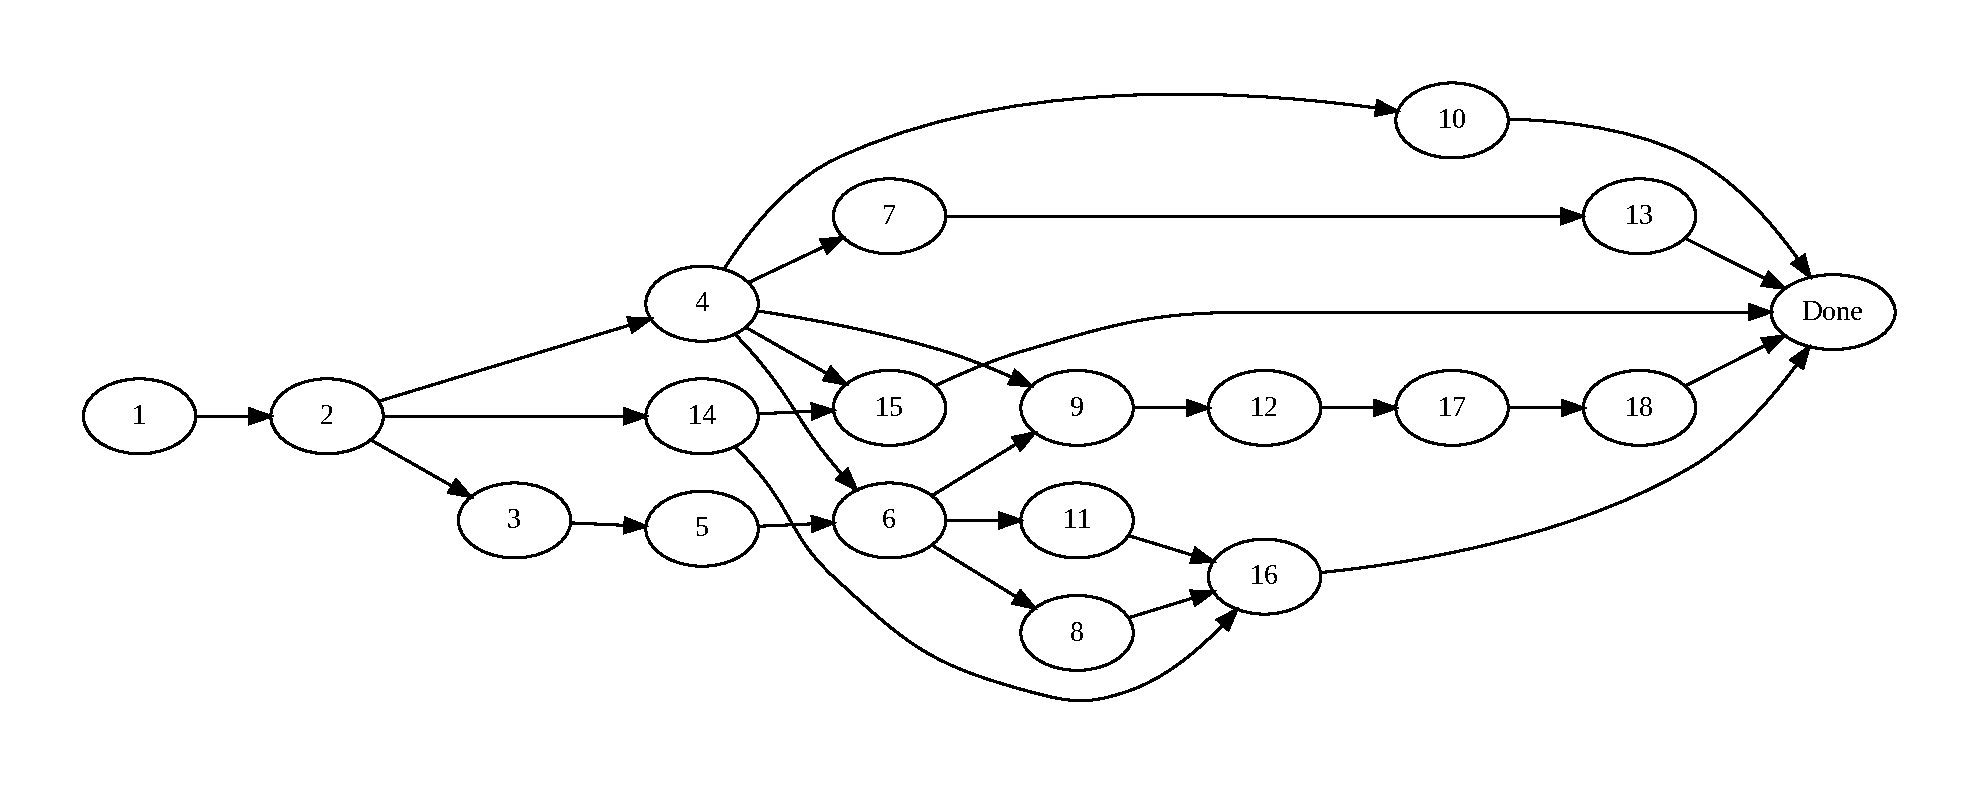
\includegraphics[width=14cm,keepaspectratio]{../figures/fig1-1}
\end{figure}

\subsection{Decision variable}

\begin{syms}
\item[$x_t$] indicates the week in which task $t\in T$ starts; $0 \leq x_t\in \Int$. For convience
    let $\vect{x} = \left( x_1, \ldots, x_t\right)^T \in \Int^n$.
\end{syms}

\subsection{Model}


\begin{mini!}
    {\vect{x}}{f\left(x_{n+1}\right)=x_{n+1} \protect\label{eq:b2-q1-obj}}{\label{eq:b2-q1}}{}
    \addConstraint{x_i}{\geq a_{ij}( x_j + d_j), \forall (i, j) \in T\times T \protect\label{eq:b2-q1-ctr1}}
    \addConstraint{x_t}{\geq 0, \forall t \in T \protect\label{eq:b2-q1-ctr2}}
\end{mini!}

The objective $f(x_{n+1})$ given by \cref{eq:b2-q1-obj} is the start time of task
with $t=19$. Since $d_{19}=0$, this also is the end time of the final task. In other
words, we week to minimize the time of completion of the entire project.

\Cref{eq:b2-q1-ctr1} simply enforces that task $i$, which starts at $x_i$ can not 
start until its predecessor $j$, which finishes at week $x_j+d_j$, is complete.
When there is no arc from $j$ to $i$, $a_{ij}=0$ and the inequality constraint is
satisfied. \Cref{eq:b2-q1-ctr1} is the canonical non-negativity constraint on $\vect{x}$.

\subsection{Results}\label{section:1.1.4}

\newpage

\section{Question 2}

\subsection{Parameters}

\begin{syms}
    \item[$T$] enumerates $n=18+1$ project tasks, ie. $T=\left\lbrace 1,\ldots,n+1\right\rbrace$

    \item[$A$] the matrix of arcs with $A\in\left\lbrace 0,1\right\rbrace^{n+1\times n+1}$;
    with elements $a_{ij}=\begin{cases}1 & \texttt{task } j \text{ preceeds }\texttt{task }i\\
    0 & \text{otherwise}\end{cases}$

    \item[$d_t$] the duration in weeks to complete task $t\in T$ with no additional labour hours allocated

    \item[$r_t$] the maximum reduction in duration of task $t\in T$ in weeks that can be 
        achieved by allocating additional labour

    \item[$c_t$] cost in $1000\euro{}$ / week when allocating additional labour
        to task $t\in T$.

    \item[$b$] bonus paid in $1000\euro{}$ per week the project finishes early; 
        with $b=30$

\end{syms}

Refer to \cref{table:1-1} for values of the above parameters.

\subsection{Decision variables}

\begin{syms}
\item[$x_t$] indicates the week in which task $t\in T$ starts; $0 \leq x_t\in \Int$. For convience
    let $\vect{x} = \left( x_1, \ldots, x_{n+1}\right)^T \in \Int^{n+1}$.

\item [$y_t$] indicates the number of weeks by which duration of task $t\in T$ is
    reduced; with $0\leq y_t \in\Int$. For convience, let
    $\vect{y} = \left( y_1,\ldots, y_n\right)^T \in \Int^n$
\end{syms}

\subsection{Model}


\begin{maxi!}
    {\vect{x}, \vect{y}}{g\left(\vect{x}, \vect{y}\right)=b\left(x_{n+1}-f_1^\star\right) \protect\label{eq:b2-q2-obj}}{\label{eq:b2-q2}}{}
    \addConstraint{x_i}{\geq a_{ij}( x_j + d_j - y_j), \forall (i, j) \in T\times T \protect\label{eq:b2-q2-ctr1}}
    \addConstraint{y_t}{\leq r_t, \forall t\in T\setminus \left(n+1\right) \protect\label{eq:b2-q2-ctr2}}
    \addConstraint{x_t}{\geq 0, \forall t\in T \protect\label{eq:b2-q2-ctr3}}
    \addConstraint{y_t}{\geq 0, \forall t\in T \protect\label{eq:b2-q2-ctr4}}
\end{maxi!}

Let $f^*$ be the optimal value of the objective function found in results for 
question 1 in \cref{section:1.1.4}, ie. the earliest time which the project can
be completed without allocating additional labour. The completion date which
maximizes the bonus paid to the countractor is given by:

$$
y_{n+1} = x_{n+1} - f_1^\star.
$$

Then the total bonus for completing the job early is given by

\begin{equation}\label{eq:b2-q2-obj1}
g\left(\vect{x}, \vect{y}\right) = b y_{n+1} = b\left(x_{n+1}-f_1^*\right).
\end{equation}

The above \cref{eq:b2-q2-obj1} is the quantity that the contractor seeks to maximize and becomes 
the objective function \cref{eq:b2-q2-obj}. \Cref{eq:b2-q2-ctr1} is similar to 
\cref{eq:b2-q1-ctr1}, in \cref{section:1.1.4}, but takes into account the reduction in duration
for the previous task. The maximum possible reduction in duration for task
$t\in T$ is limited by $r_t$. This is represented by the family of constraints
in \cref{eq:b2-q2-ctr2}. \Cref{eq:b2-q2-ctr3} and \cref{eq:b2-q2-ctr4} are simply
the family of canonical non-negativity constraints on decision variables
$\vect{x}$ and $\vect{y}$.

\subsection{Results}
